\chapter{The Language of Quantum Information Theory}
% Section on density operator
\section{Density Operators}
%%%%%%%%%%Postulates of Quantum Mechanics
\subsection{Postulates of Quantum Mechanics}
We begin by stating the a common axiomatization of Quantum Mechanics (QM) based on Hilbert Spaces following \cite{ballentine_quantum_2014}, we choose it for mathematical simplicity; for alternatives see e.g. \cite{reyes-lega_aspects_2015}.
\begin{enumerate}
        \item To each physical system $\mathcal{S}$ there corresponds a separable Hilbert Space $\mathcal{H}$ such that states of the system are described by positive and unit trace operators on it. The Hilbert Space of a composite system made up of $\mathcal{S}$ and $\mathcal{S}'$
        is given by the tensor product of the Hilbert spaces $\mathcal{H}\otimes\mathcal{H}'$.
        \item To each dynamical variable there corresponds a self-adjoint operator on $\mathcal{H}$, called an observable, whose possible
        values are given by its eigenvalues.
        \item Given a system in  state $\rho$ and some observable $A$ of it, the probability of measuring $A$ and obtaining the result
        $\lambda$ is given by $\mathrm{Tr}[\rho P_{\lambda}]$ where $P_{\lambda}$ is the eigen-projector into the subspace associated with
        $\lambda$. Furthermore the expectation value is $\mathrm{Tr}[\rho A]$.
        \item After a measurement with result $\lambda$ the state of the system becomes $\frac{P_{\lambda}\rho P_{\lambda}}{\mathrm{Tr}[P_{\lambda}\rho
        P_{\lambda}]}$.
        \item The time evolution of the system in a time interval $(0,t)$ in which no measurement is done is given by some unitary operator
        $U_{t}$ according to $\rho_{t}=U_{t}\rho U_{t}^{\dagger}$ where $\rho$ is the state of the system at time $t=0$.
\end{enumerate}
Operators satisfying the properties required for a state are called \textit{\textbf{Density Operators}} and in contrast to frameworks
whose treatment of quantum states is merely as rays in $\mathcal{H}$, they describe statistical mixtures so imperfect state preparation
can be handled. To see this consider the spectral resolution of some density operator:
\begin{equation}
  \rho = \sum_{n}p_{n}\ketbra{\psi_{n}}
\end{equation}
by definition we have $p_{n}\geq 0, \sum_{n}p_{n}=1$  any density operator can be seen as a convex sum of rays in $\mathcal{H}$ (provided we
identify each one with its associated projector $\ketbra{\psi}$) and from it an  interpretation of $\rho$ as an statistical mixture of rays is
suggested: given a preparation process, there is a probability $p_{n}$ for the system to be in the state $\ketbra{\psi_{n}}$ after it, for this
reason states of the form $\ketbra{\psi}$ are called \textbf{\textit{Pure}} while those who are not we refer to as \textbf{\textit{Mixed}}.
This \textbf{\textit{Ensemble Interpretation}} has serious conceptual challenges when one tries to use it outside a
fixed preparation procedure due to the non-uniqueness of the decomposition into pure states \cite{nielsen_quantum_2010},
but is good enough for the porposes of the present work, for a comprehensive discussion of this
topic the reader is refered to \cite{schlosshauer_decoherence_2007}.
%%%%%%%%%%%%%%Time evolution
\subsection{Time Evolution}
Assuming the evolution to be differentiable in time, we have that there exists a self-adjoint operator $H$ such that $U_{t} = \mathrm{exp}(-itH)$
\footnote{Unless otherwise stated, from here on we assume $\hbar=1$}, called the \textbf{\textit{Hamiltonian}} of the systems and which
acts as the generator of the dynamics. It is straightforward now to construct a differential equation for $\rho_{t}$ by taking the derivative
of it:

\begin{align}
  \rho_{t}=& e^{-itH}\rho_{t}  e^{itH}\\
  \partial_{t}\rho_{t} =& -iH\rho_{t} + \rho_{t}iH\\
  \partial_{t}\rho_{t} =& -i[H, \rho_{t}]\label{eq:Liouville-VonNeumann}.
\end{align}
Equation \eqref{eq:Liouville-VonNeumann} is called the Liouville-Von Neumann equation, it generalizes the  Schr\"{o}dinger equation
to mixed states and can be interpreted as the quantum analog of the Liouville equation in classical mechanics (with the Poisson braket) through
the quantization rule $\{\bullet,\bullet\} \to -i[\bullet,\bullet]$. As will be seen in later chapters, this type of evolution is characteristic
of closed quantum systems.
%%%%%%%%%%Purity
\subsection{Purity}
Say we got a particular state production processes whose product $\rho$ we characterize via say tomography \cite{nielsen_quantum_2010}, it
becomes immedeatley important to quantify to which extent we can regard the product as being composed of only one pure states
(hopefully the one we wanted to prepare) i.e. we want to define the purity of the state, with this motivation one look for a map
$\mathcal{E}$ from the space of density operators to the reals such that:
\begin{itemize}
        \item $\mathcal{E}(\rho)$ is maximal if and only if $\rho$ is pure.
        \item it is conserved under unitary evolution.
\end{itemize}
The first one makes this map a figure of merit one can try to maximize and the second one is imposed to assure that it doesn't changes in a
closed system unless a measurement is made, as allowing the free evolution of the system should not improve the knowledge of the
experimenter about the system. The standard choiche (altough not the only one) is the \textit{\textbf{Purity}},
defined as \cite{nielsen_quantum_2010, ballentine_quantum_2014}:
\begin{definition}
The purity $\gamma$ of a state $\rho$ is:
  \begin{equation}
    \gamma = \Tr{\rho^{2}}.\label{eq:definition_purity}
  \end{equation}
\end{definition}
The requirements are quickly checked:
\begin{align}
  \Tr{\rho^{2}_{t}} =& \Tr{(U_{t}\rho_{0}U_{t}^{\dagger})(U_{t}\rho_{0}U_{t}^{\dagger})} = \Tr{\rho_{0}^{2}}\\
  \Tr{\rho^{2}} =& \sum_{n}p_{n}^{2} \leq 1
\end{align}
in the second line the inequality is saturated if and only if $\rho=\ketbra{\psi}$.
\section{Entanglement}
One of the key differences between the structure of the state space of classical and quantum systems is the existance
of non-separable states when considering multipartite systems \cite{reyes-lega_aspects_2015,diosi_short_2011,nielsen_quantum_2010} which allows
the latter to have new a new type of correlations. Here we define entanglement for mixed states following \cite{diosi_short_2011}:

\begin{definition}
  Given a state $\rho$ in a system composed of two subsystems $A$ and $B$ with total Hilbert space $\mathcal{H}_{A}\otimes \mathcal{H}_{B}\}$, we say it is
  an \textbf{\textit{entangled}} or \textit{\textbf{non-separable}} if there doesn't exists a set states $\{\rho_{j}\otimes \sigma_{j}\}_{j}$ and coefficients
  $\{p_{j}\}_{j},  \sum_{j}p_{j}=1, \hspace{0.1cm} p_{j}\geq 0$ such that:
  \begin{equation}
    \rho = \sum_{j}p_{j}\rho_{j}\otimes \sigma_{j}
  \end{equation}
  if it does exists, the state is called \textbf{\textit{separable}}.
\end{definition}
For the case of pure state this definition coincides with the usually given one \cite{nielsen_quantum_2010}: say $\rho=\ketbra{\psi}$ is pure and separable, then:
\begin{equation}
  \Tr{\rho^{2}} = \sum_{jk}p_{j}p_{k}\Tr{\rho_{j}\rho_{k}}\Tr{\sigma_{j}\sigma_{k}}
\end{equation}
and by the Cauchy-Schwartz inequality with the Frobenious inner product
\begin{equation}
  \Tr{\rho^{2}} \leq \sum_{jk}p_{j}p_{k}\Tr{\rho_{j}^{2}}\Tr{\rho_{k}^{2}}\Tr{\sigma_{j}^{2}}\Tr{\sigma_{k}^{2}} \leq 1
\end{equation}
the first inequality from right to left saturates if and only if all the $\rho_{j}$ and $\sigma_{k}$ are pure, and the first one if
and only if all the $\rho_{j}$ and $\sigma_{k}$ are equal between themselves i.e. $p_{j}=\delta_{0j}$, hence there are pure states
in $\mathcal{H}_{A}$ and $\mathcal{H}_{B}$ such that:
\begin{equation}
  \ketbra{\psi} = \ketbra{\alpha}\otimes\ketbra{\beta}.
\end{equation}
For a classical system all states are separable thanks to the representation via $\delta$ functions
of probability densities \cite{diosi_short_2011} and in this sense entanglement is a purely non-classical phenomena, in fact for pure states
this completely exhaust all the possible non-classical correlations. For mixed states the characterization is considerably richer
and allows for bipartite states that despite being separable show non-classical correlations \cite{adesso2016introduction}.
\subsection{Marginalization}
Consider a bipartite system in state $\rho$ with subsystems $A$ and $B$, and assume only the former can be accessed
experimentally; e.g. $B$ is on the other side of the galaxy, has too many degrees of freedom or is simply not of interest and is desirable
to prescend from it. Any
observable $\Gamma$ that we decide to measure must be of the form $\Gamma=\Lambda \otimes I$ so that it describes only actions on
$\mathcal{H}_{A}$; in this sense we say it is \textit{\textbf{local}}. We want to obtain the probability distribution describing the statistics
of $\Lambda$, by definition:
\begin{align}
  \wp(\lambda)=&\Tr{\rho (\ketbra{\lambda^{A}}\otimes I)}\\
  \wp(\lambda)=& \sum_{\lambda'k}\bra{\psi_{k}^{B}}\bra{\lambda'^{A}}\rho (\ketbra{\lambda}\otimes I)\ket{\lambda'^{A}}\ket{\psi_{k}^{B}}\\
  \wp(\lambda)=& \sum_{\lambda'k}\bra{\psi_{k}^{B}}\bra{\lambda'^{A}}\rho \ket{\lambda'^{A}}\ket{\psi_{k}^{B}} \delta_{\lambda\lambda'}\\
  \wp(\lambda)=& \sum_{k}\bra{\psi_{k}^{B}}\bra{\lambda^{A}}\rho \ket{\lambda^{A}}\ket{\psi_{k}^{B}} \\
  \wp(\lambda)=&\bra{\lambda^{A}} \left(\sum_{k}\bra{\psi_{k}^{B}}\rho\ket{\psi_{k}^{B}}\right)\ket{\lambda^{A}}\\
  \wp(\lambda)=& \Tr{\ketbra{\lambda^{A}}\sum_{k}\bra{\psi_{k}^{B}}\rho\ket{\psi_{k}^{B}}} \label{eq:partial_trace}.
\end{align}
Equation \eqref{eq:partial_trace} suggest that there exists a state in $\mathcal{H}_{A}$ whose statistics  coincide
with those of $\rho$ and that it should be given by the sum in \eqref{eq:partial_trace}, in this sense we have a marginalization i.e.
an assignement of states of in $\mathcal{H}_{A}\otimes\mathcal{H}_{B}$ to states in $\mathcal{H}_{A}$ such that it has the correct statistics
i.e. $\Tr{\rho^{AB}(\Lambda \otimes I)}=\Tr{\rho^{A}\Lambda}$ for any observable $\Lambda$ of $A$. It is desirable for this map to be unique
for the following: assume an experimentalist has an infinite ensemble of copies of the system in state $\rho$ but can only measure local
observables in $A$, although any and as many time as wanted, i.e. it is possible to fully characterize the statistics of any local observable,
which state should the experimentalist asign? If the marginalization is not unique there is an ambiguity, an marginalizations sure must
exists as local experiments are always possible, hence uniqueness is important to account properly for this experiment; turns out to
assure it suffices to demand linearity. This map is called the \textit{\textbf{Partial Trace}}:

\begin{definition}
  Given two vector spaces $V$ and $W$, for simplicity assumed of finite dimension\footnote{although we will use it too for infinite dimensions without inquiring wheter the operators are even traceclass}, the partial trace taken over $W$ is the map\cite{nielsen_quantum_2010}:
\[
\mathrm{Tr}_{W}: \begin{array}{rcl}
A\otimes B \in \mathcal{L}(V\otimes W)& \mapsto & A \Tr{B} \in \mathcal{L}(V)
\end{array}
\]
where the $\mathcal{L}$ denotes the space of operator, and the map is  linearly extended to all of $\mathcal{L}(V\otimes W)$
.
\end{definition}
The linear extension makes the partial trace coincide with the sum in \eqref{eq:partial_trace} and the non-manifestly base invariant definition
usually given in sources like \cite{maziero2017computing}. Next we prove this is in fact the only linear map with the correct statistics:
\begin{theorem}
  The partial trace is the only linear map such that $\mathcal{E}:\to \mathcal{L}(\mathcal{H}_{A}\otimes \mathcal{H}_{B}) \to \mathcal{L}(\mathcal{H}_{A})$
  such that $\Tr{\rho (\Lambda\otimes I)} = \Tr{\mathcal{E}(\rho)\Lambda}$ for all $\rho \in \mathcal{H}_{A}\otimes \mathcal{H}_{B}$ and
  $\Lambda \in \mathcal{L}(\mathcal{H}_{A})$.
\end{theorem}
\begin{proof}
  Assume there exists a map $\mathcal{E}:\to \mathcal{L}(\mathcal{H}_{A}\otimes \mathcal{H}_{B}) \to \mathcal{L}(\mathcal{H}_{A})$ with the
  correct statistics and introduce an orthogonal product basis in $\mathcal{H}_{A}\otimes \mathcal{H}_{B}$,
  $\{\ket{\psi^{A}_{j}}\ket{\psi^{B}_{k}}\}_{jk}$. By construction we have:
  \begin{align}
    \Tr{\mathcal{E}(\rho)\Lambda} =& \sum_{jk} \bra{\psi^{B}_{j}}\bra{\psi^{A}_{k}}\rho (\Lambda \otimes I) \ket{\psi^{A}_{k}}\ket{\psi^{B}_{j}}\\
 \Tr{\mathcal{E}(\rho)\Lambda} =& \sum_{k} \bra{\psi_{k}^{A}}\sum_{j}\bra{\psi^{B}_{j}}\rho\ket{\psi^{B}_{j}}(\Lambda \ket{\psi_{k}^{A}})\\
\Tr{\mathcal{E}(\rho)\Lambda} =& \sum_{k} \bra{\psi_{k}^{A}}\Trp{B}{\rho}(\Lambda\ket{\psi_{k}^{A}})\\
\Tr{\mathcal{E}(\rho)\Lambda} =& \Tr{\Trp{B}{\rho}\Lambda}\\
  \end{align}
  As this holds for any $\Lambda$ and $\rho$, we have that $\mathcal{E}=\mathrm{Tr}_{B}$.
\end{proof}
Note that in the above proof we have not used any properties of $\rho$ or $\Lambda$ unlike in \eqref{eq:partial_trace}. A few remarks are
in order:
\begin{enumerate}
  \item The partial traces of an state $\rho \in \mathcal{L}(\mathcal{H}_{A}\otimes\mathcal{H}_{B})$ are always mixed, unless $\rho$ is
        both pure and separable. In this sense we say the subsystems of a system in an entangled state can not be perfectly known, not even if
        the state of the complete system is perfectly known \autocite{nielsen_quantum_2010, adesso2016introduction, diosi_short_2011}.
  \item When $\rho$ is entangled and pure $\Trp{B}{\rho}$ is an improper mixture \cite{schlosshauer_decoherence_2007}, in the sense that for none of the possible ensembles that
        represent this density operator is possible to say that $A$ is in an unknown state $\ket{\psi} \in \mathcal{H}_{A}$  with some
        probability; if this were the case we could perform experiments in both $A$ and $B$ to discover this unknown states and then the total
        state would have not been entangled in the first place.
  \item For identical particles this construction is not valid as the space of physical states is not $\mathcal{H}_{A}\otimes \mathcal{H}_{B}$
        but its symmetrization, otherwise the symmetrization postulate is violated.
        For proposals of suitable generalizations see \cite{reyes-lega_aspects_2015}.
\end{enumerate}
Despite this conceptual difficulties the partial trace remains a key tool in Quantum Information Theory for studying open systems and
local operations.
\section{Quantum Operations}
Now that we have means of describing unitary evolutions and marginalizations we are in a position to describe the most general class
of transformation a quantum system can undergo, the so called \textbf{\textit{Quantum Operations}}. In general we can describe any
evolution of a system of interest ($S$), called from here on simply \textbf{\textit{the system}}, by asumming there exists another one called
\textbf{\textit{the environment}} ($E$) that represents the rest of the universe, and whose degrees of freedom are undesirable in the
description of the $S$; these scheme is called \textit{\textbf{S+E}} and the total hamiltonian is generically of the form
$H = H_{S}\otimes I + I\otimes H_{E} + V$ where the coupling between the two is given by the last term \cite{wiseman_quantum_2010};
for simplicity it is assumed the environment and the system are distinguishable \cite{breuer2002theory}. The whole point is this
is to construct a non-unitary map describing the evolution of $S$ by evolving unitarily the whole and tracing over the environment:

\begin{equation}
 \mathcal{E}_{t}(\rho_{0}) \equiv \Trp{E}{U_{t}\left(\rho_{0}\otimes \sigma\right)U_{t}^{\dagger}} = \rho_{t}
\end{equation}
\begin{figure}[h]
 \centering
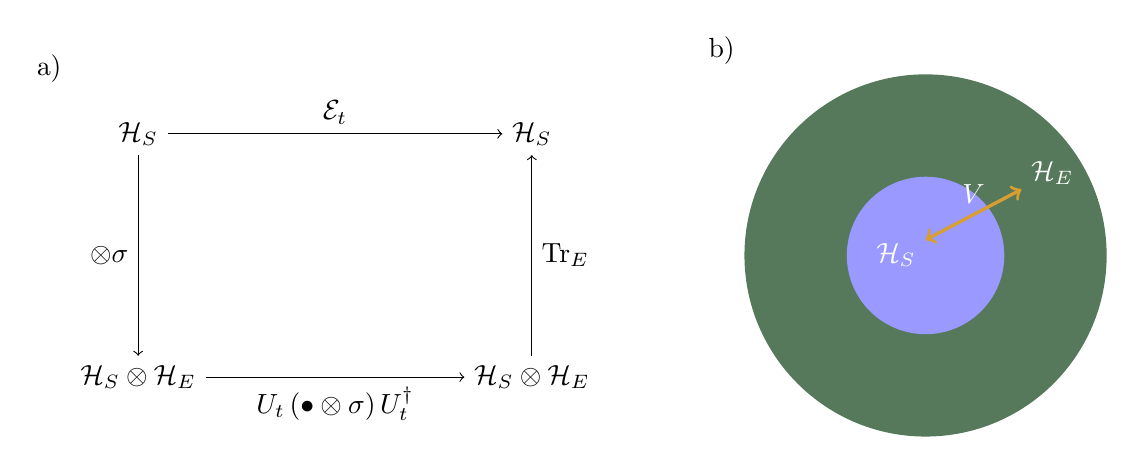
\begin{tikzpicture}%[transform canvas={scale=1.3}]
% Define colors
\definecolor{colorenv}{HTML}{55795A}
\definecolor{colorsys}{HTML}{7286D3}
\definecolor{colorarrow}{HTML}{D99E30}

  %%%%%%%%%%%%%%%%%5Commutation diagram
  % Define nodes
  \begin{scope}[local bounding box=drawA]
  \node (A) at (0cm,0) {$\mathcal{H}_{S}$};
   \node (B) at (5cm,0) {$\mathcal{H}_{S}$};
  \node (C) at (0cm,-3.09cm) {$\mathcal{H}_{S}\otimes\mathcal{H}_{E}$};
  \node (D) at (5cm,-3.09cm) {$\mathcal{H}_{S}\otimes\mathcal{H}_{E}$};
  % Draw arrows
   \draw[->] (A) -- (B) node[midway, above] {$\mathcal{E}_{t}$};
  \draw[->] (A) -- (C) node[midway, left] {$\otimes \sigma$};
  \draw[<-] (B) -- (D) node[midway, right] {$\mathrm{Tr}_{E}$};
  \draw[->] (C) -- (D) node[midway, below] {$U_{t}\left(\bullet\otimes\sigma\right)U_{t}^{\dagger}$};
\end{scope}
\node[above left] at (drawA.north west) {a)};
  \begin{scope}[local bounding box=drawB]
  %%%%%%%%%%The circles
  %Circles
  \fill[color=colorenv] (10cm,-1.545cm) circle (2.3cm);

  \fill[blue!40] (10cm,-1.545cm) circle (1cm);
  %Marks
  \node[text=white, anchor=east] (E) at (10cm,-1.545cm) {$\mathcal{H}_{S}$};
  \node[text=white, anchor=east] (F) at (12cm,-0.5cm) {$\mathcal{H}_{E}$};
   \draw[<->, line width=1.2pt, color=colorarrow, text=white] (E) -- (F) node[midway, above] {$V$};
  \end{scope}
 \node[above left] at (drawB.north west) {b)};
\end{tikzpicture}
\end{figure}
%%%%%%%%%%%%%%%%%%%%%%%%%%%%%%%%%%%%%%%%Von Neumann Entropu
% \subsection{The Von Neumann Entropy}
% As can be seen in the study of Bell's inequalities in a two qubit system, not all entangled states show the same amount of violation of the
% inequalities, and it is not even true that non-separability is sufficient to violate them \cite{ballentine_quantum_2014}, thus not all entangled
% states are made equal and classifying them is a relevant task; to achieve this we introduce \textit{\textbf{Entanglement Measures}}, which
% quantify how strong this non-classical correlations is in a bipartite state.
% Following \cite{vedral1997quantifying} we demand from any proper measure:

% \begin{enumerate}
%         \item it is a map $\mathcal{E}:\mathcal{L}(\mathcal{H}_{A}\otimes\mathcal{H}_{B}) \to \mathds{R}^{+}$.
%         \item $\mathcal{E}(\rho)=0$ if and only if $\rho$ is separable.
%         \item Local unitary operations preserve $\mathcal{E}(\rho)=\mathcal{E}(U_{A}\otimes U_{B} \rho U_{A}^{\dagger}\otimes U_{B}^{\dagger} )$.
%   \item The entanglement can not be increased via classical communication or local measurements \footnote{for proper definitions of
%         these see \cite{diosi_short_2011, vedral1997quantifying}}.
% \end{enumerate}
% The first condition is just the basic requirement for a figure of merit, the second assures the measure identifies the absence of entanglement,
% and the last two that the two systems can not become correlated via operations that pertain to only one of them.
%%% Local Variables:
%%% mode: latex
%%% TeX-master: "../main"
%%% End:
